\documentclass[Experiments]{subfiles}
\begin{document}
\section{Experiments}

\label{sec:Measurements}
% TODO: Needed better introduction
% Lutz: Feitelijk is dit allemaal herhaling van dingen uit het vorige hoofdstuk. In principe kan je dus zeggen, dat dit hoofdstuk de daadwerkelijke metingn documenteerd, zoals die in het vorige hoofdstuk geschetst werden. 
Basically, there are two main different scenarios for measuring the performance. The first one is by measuring the performance of Nginx when Naxsi is disabled. The second one is by measuring the performance when Naxsi is enabled.  First, a baseline measurement is performed with a Wordpress website on the back-end server. Second, the performance baseline is measured where Nginx only returns a \verb+HTTP 200 OK+ response. The latter baseline measurement gives the lowest overhead and maximum performance of the Nginx webserver.

\subsection{Baseline performance measurements}

\subsubsection{Wordpress}
\label{sec:Baseline performance measurement}
In order to measure the performance of Naxsi, it is important to know the bottleneck of the back-end server processing all the application logic. Table~\ref{fig:Baseline measurement 1} shows that $\approx 21~\%$ of the 10,000 requests produce a \verb+HTTP 5xx+ response when using 250 concurrent connections. Details can be found in appendix \ref{sec:baseline_measurement_1}.

\begin{table}[H]
\caption{httperf measurement 1}
\begin{tabular}{|p{2cm}|p{1,5cm}|p{1,5cm}|p{1,5cm}|p{1,5cm}|p{1,5cm}|}
\hline
 & \textbf{1xx} & \textbf{2xx} & \textbf{3xx} & \textbf{4xx} & \textbf{5xx} \\ \hline
\textbf{Connections} & 0 & 0 & 8542 & 0 & 1458 \\ \hline
\end{tabular}
\label{fig:Baseline measurement 1}
\end{table}

By using a half-interval search method, the optimal number of concurrent connections is found, which gives the highest rate of 190 request per second. As can be seen in figure~\ref{fig:Baseline measurement 2}, the total number of \verb+HTTP 3xx+ responses is 10,000. Details can be found in appendix~\ref{sec:baseline_measurement_2}.

\begin{table}[H]
\caption{httperf measurement 2}
\begin{tabular}{|p{2cm}|p{1,5cm}|p{1,5cm}|p{1,5cm}|p{1,5cm}|p{1,5cm}|}
\hline
 & \textbf{1xx} & \textbf{2xx} & \textbf{3xx} & \textbf{4xx} & \textbf{5xx} \\ \hline
\textbf{Connections} & 0 & 0 & 10000 & 0 & 0 \\ \hline
\end{tabular}
\label{fig:Baseline measurement 2}
\end{table}

Based on the values derived from the measurement above, the performance is measured by stepping through the concurrent connections from 1 to 200. The response time is calculated by taking the average of each measurement of  each step. Each step has a measurement duration of 60 seconds. When staying under $190$ concurrent connections, the response time is \mbox{$\approx 30 ms$}. The resource usage on server01 is very minimal, of which the details can be found in appendix~\ref{sec:Wordpress baseline resource usage}.

% autobench --single_host --host1 wp_without_naxsi.test.nl --uri1 /index.php --low_rate 1 --high_rate 230 --rate_step 1 --num_call 1 --const_test_time 60 --file results.csv
\begin{figure}[H]
\caption{Wordpress baseline measurement}
\centering
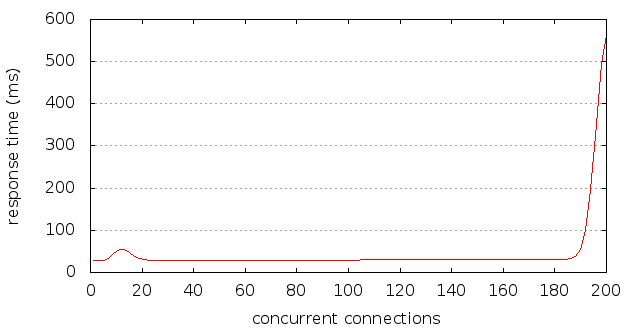
\includegraphics[scale=0.55] {images/results/baseline_wp/output.png}
\label{fig:Baseline performance measurement}
\end{figure}

\subsubsection{HTTP 200 OK}
To measure the performance of the Nginx web server, the number of concurrent connections is incremented with steps of 10. Figure~\ref{fig:HTTP 200 OK: requests per second} shows some erratic behaviour when looking at the number of request per second that is measured. This is because the number of requests per second is relatively high and Apache benchmark is not capable of measuring consistent results. The gray line shows the lowest measured value and the highest measured value. The red line shows the average value for each step. The maximum number of requests per second is $11,973$, which is reached when $380$ concurrent connections are used. Therefore, 380 concurrent connections is considered as the optimal number of concurrent connections for this configuration. The resource usage of server01 can be found in appendix~\ref{sec:HTTP 200 OK baseline resource usage}.

\begin{figure}[H]
\caption{HTTP 200 OK: requests per second}
\centering
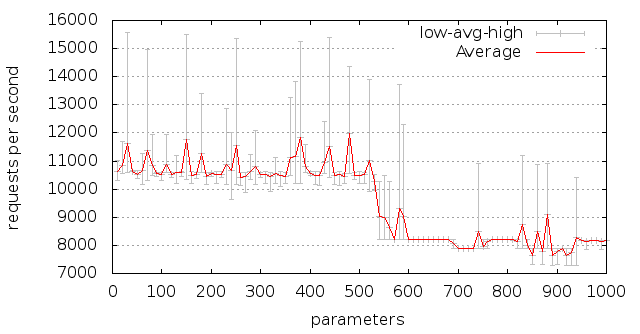
\includegraphics[scale=0.55] {images/results/baseline_200/output.png}
\label{fig:HTTP 200 OK: requests per second}
\end{figure}

\subsection{Performance measurements with Naxsi}

\subsubsection{Wordpress}

\paragraph*{Allowed parameters}

Figure~\ref{fig:wordpress_with_naxsi_valid_parameters} shows how the response time evolves when the number of valid \ac{URL} parameters increases. As determined during the baseline measurements, the number of optimal concurrent connections is $190$. Each measurement is performed with the same number of concurrent connections, but the number of \ac{URL} parameters are increased. As can been seen in figure~\ref{fig:wordpress_with_naxsi_valid_parameters}, when 20 parameters are used, the response time is $0.8$ milliseconds longer than when no parameters are used.

\begin{figure}[H]
\caption{Valid URL parameters}
\centering
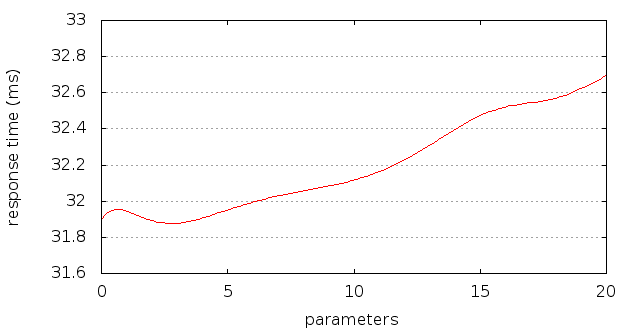
\includegraphics[scale=0.55] {images/results/wp_with_naxsi_incremented_allowed_parameters/output.png}
\label{fig:wordpress_with_naxsi_valid_parameters}
\end{figure}

\paragraph{Disallowed parameters}

At first sight, the graph in figure~\ref{fig:Invalid parameters} shows strange behaviour. This is because as soon as Naxsi sees an invalid \ac{URL} parameter, it returns an \verb+HTTP 403+ error code to the requesting client. The first measurement, where no \ac{URL} parameter is used, the requests gets forwarded to the back-end server that processes the request, and the results get back to the client. This takes about the same amount of time as is measured during the baseline measurements. As soon as an \verb+HTTP 403+ error code is returned, it takes only very little time, as can be seen in table~\ref{tab:Wordpress response time with invalid URL parameters}.

\begin{table}[H]
\caption{Wordpress response time with invalid URL parameters}
\center
\begin{tabular}{|r|r|}
\hline
\textbf{Parameters} & \textbf{Response time (ms)}\\ \hline
0 & 31.7 \\ \hline
1-5 & 0.3 \\ \hline
6-17 & 0.4 \\ \hline
18-20 & 0.5 \\ \hline
\end{tabular}
\label{tab:Wordpress response time with invalid URL parameters}
\end{table}

\begin{figure}[H]
\caption{Invalid URL parameters}
\centering
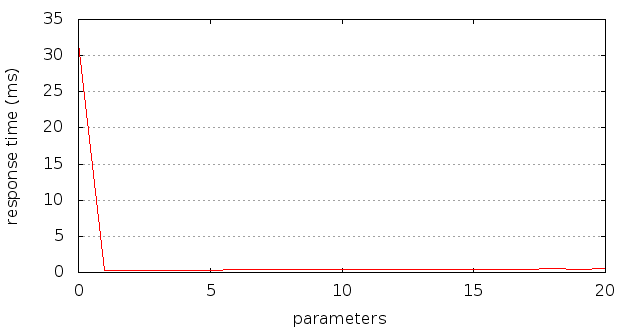
\includegraphics[scale=0.55] {images/results/wp_with_naxsi_incremented_disallowed_parameters/output.png}
\label{fig:Invalid parameters}
\end{figure}

\subsubsection{HTTP 200 OK}

\paragraph{Allowed parameters}
Although, the influence on the response time caused by the number of \ac{URL} parameters is already visible during the Wordpress measurements, it is much more visible when the Nginx server only returns  \verb+HTTP 200 OK+ responses, as can be seen in figure~\ref{fig:HTTP 200 OK: valid url parameters}. The number of requests per seconds decrease somewhat linearly when the number of \ac{URL} parameters increase. When 20 \ac{URL} parameters are used, the number of requests per second drop with $\approx 35\%$ compared to when no parameters are used.

\begin{figure}[H]
\caption{Valid URL parameters}
\centering
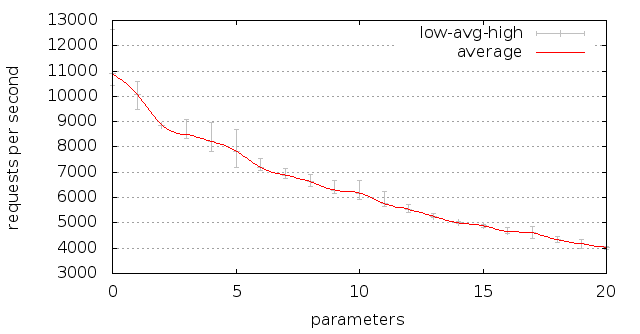
\includegraphics[scale=0.55] {images/results/200_with_naxsi_incremented_allowed_parameters/output.png}
\label{fig:HTTP 200 OK: valid url parameters}
\end{figure}

\paragraph{Disallowed parameters}
When Naxsi allows the request to be further processed, then Nginx returns an \verb+HTTP 200 OK+ response the client. When Naxsi denies a request, then Nginx returns an \verb+HTTP 403+ error code to the client. In both cases, there is no processing overhead when returning an HTTP code. Although the line in figure~\ref{fig:HTTP 200 OK: invalid url parameters} proceeds similar to the one in figure~\ref{fig:HTTP 200 OK: valid url parameters}, it shows, that denying a request comes with some extra performance loss. The number of requests per second do not decrease linearly, however, but they appear to converge to the same number of requests per second as would be the case when only valid \ac{URL} parameters are used. When comparing the measurements of both valid \ac{URL} parameters and invalid \ac{URL} parameters, the number of concurrent requests per second is approximately 1,000 requests less when 10 parameters are used of which the last \ac{URL} parameter has bad content.

\begin{figure}[H]
\caption{Invalid URL parameters}
\centering
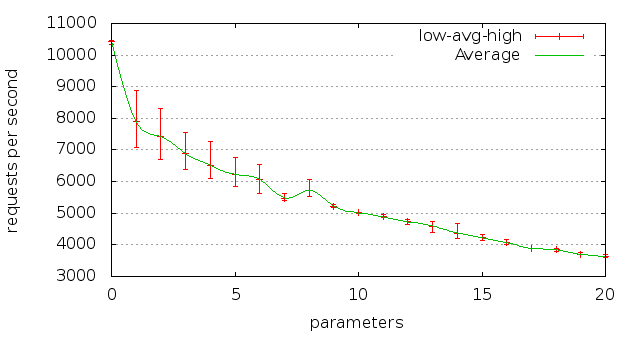
\includegraphics[scale=0.55] {images/results/200_with_naxsi_incremented_disallowed_parameters/output.png}
\label{fig:HTTP 200 OK: invalid url parameters}
\end{figure}

\end{document}
